\chapter{Altri formalisimi e Macchine di Turing}

\section{Formalismi totali e problema dell'interprete}

Ci sono varie estensioni possibili al formalismo primitivo ricorsivo. Un esempio è il sistema T di
Gödel, che aggiunge l'ordine superiore. Questo ci permette di scrivere la funzione di Ackermann.
Un'altra possibilità è quella di rilassare la ricorsione primitiva permettendo una ricorsione che
permetta di andare in ricorsione su ordinamenti ben fondati. Questa condizione è verificabile in
termini sintattici, entro certi limiti.

Esteso il mio linguaggio ottengo la possibilità di scrivere la funzione di Ackermann e le mie
funzioni sono totali. Sono complete? O c'è qualche funzione totale che posso pensare ma non
scrivere? C'è una dimostrazione che dice che sì, tutti questi formalismi saranno incompleti. Un
formalismo che permette di scrivere solo programmi terminanti sarà sempre incompleto.

La dimostrazione è abbastanza semplice. L'idea è che un programma che non riesco a scrivere (tra
i tanti) è l'interprete per il linguaggio stesso. 

Cosa intendiamo per interprete? Qui parliamo sempre di funzioni da $\Nat$ a $\Nat$. Dovremmo quindi
definire l'interprete in questi termini.

L'input dell'interprete non è un programma in senso astratto. Prende in input una stringa che
esprime il programma. Questa stringa può essere letta come un numero. Dire che una funzione è
calcolabile è equivalente a definire l'interprete per tale funzione, se vogliamo dare una
definizione operativa.

Sia data una enumerazione effettiva (e.g. lessicografica) $P_{n}$ dei programmi del
linguaggio $\Lang$, e sia $\phi_{n}$ la funzione calcolata dal programma $P_{n}$.

$P_{n}$ è un livello intensionale, una descrizione di una funzione. $\phi_{n}$ è la funzione
calcolata dal programma $n$-esimo.

Un interprete per $\Lang$ è una funzione che preso in input l'indice $n$ di un programma ed un
input $m$ simula il comportamento di $P_{n}$ su tale input, cioè una funzione $I$ tale che
\begin{equation*}
    I (n, m) = \phi_{n}(m)
\end{equation*}

Se la numerazione dei programmi è effettiva, $I$ è intuitivamente calcolabile.

È fondamentale la numerazione: dato $n$ devo poter sapere qual'è la funzione $n$-esima da interpretare.

Ci chiediamo se l'interprete per $\Lang$ può essere scritto in $\Lang$, cioè se esiste $u$ tale
che $I = \phiu$.

La risposta è no. Supponiamo infatti che esista $u$ tale che $I(n, m) = \phiu(n, m) = \phi_{n}(m)$.
Consideriamo la funzione
\begin{equation*}
    f(x) = \phiu(x,x) + 1 = \phix(x)+1
\end{equation*}

Se il linguaggio $\Lang$ è chiuso per composizione $f \in \Lang$, e dunque deve esistere un
programma $i$ tale che $\phii = f$.

Ma allora
\begin{equation*}
    \phii(i) = f(i) = \phii(i) + 1
\end{equation*}
che è assurdo

L'argomento è sempre diagonale. Mi muovo sulla digaonale mentre sui lati ho due infinità (numero
dei programmi e lunghezza dei programmi ad esempio).

L'interprete è un esempio di funzione intuitivamente calcolabile ma non esprimibile in un formalismo
totale. Tipicamente è sempre possibile, dato un linguaggio che esprime funzioni totali, trovare un
linguaggio più espressivo.

\begin{thm}
    Nessun formalismo totale è in grado di esprimere il proprio interprete.
\end{thm}

La completezza algoritmica è un concetto obsoleto. Gli algoritmi a cui siamo spesso interessati sono
quelli polinomiali in complessità. A questo punto, perché non restringersi a linguaggi di
programmazione che permettono di scrivere solo programmi con questa complessità? Si può fare, ce ne
sono tanti di linguaggi del genere, basta imporre i giusti vincoli sul linguaggio.

Da un punto di vista operativo si perde in praticità. Ma questo è anche legato al capire la
complessità computazionale dell'algoritmo. Se però si capisce bene perché un dato algoritmo ha
una certa complessità allora possiamo strutturare il programma che lo realizza in modo che rispetti
i vincoli del linguaggio. Il nostro approccio è al contrario: scriviamo i programmi e poi li
analizziamo. Questo approccio non ci dà un granchè di informazioni. Non abbiamo alcun metodo
generalizzato che ci dia informazioni o garanzie su programmi. Sarebbe più bello avere queste
informazioni a priori.

Nei linguaggi di programmazione comuni (C, Python, ecc.) posso scrivere l'interprete per il
linguaggio stesso. Perché? Perché non ho garanzie di terminazione ($\phii(i)$ divergerebbe).

Abbiamo una gerarchia nota dei linguaggi totali. Un'interessante caratterizzazione del sistema T è
che le funzioni calcolabili in questo sistema sono esattamente quelle calcolabili nell'aritmetica di
Peano al primo ordine.

\begin{figure}[h]
    \centering
    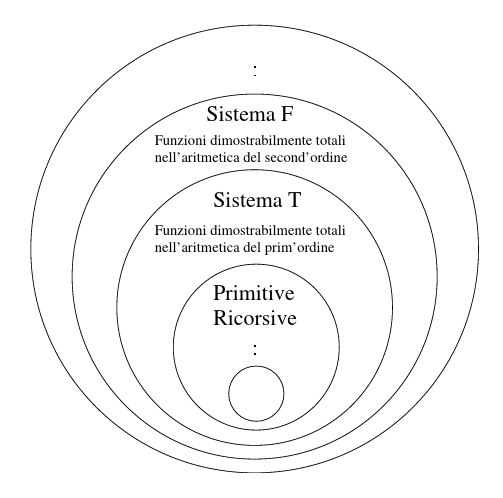
\includegraphics[scale=0.5]{img/TotalHierarchy.jpg}
    \caption{Gerarchia dei formalismi totali}
\end{figure}

\section{Tesi di Church}

Che succede se rinunciamo a questa idea della totalità? Sappiamo che non daremo luogo a paradossi.
Tuttavia rimane il problema: siamo nella situazione dei formalismi totali, e cioè esiste una
gerarchia di formalismi più potenti, o colpiamo un upper bound tale che in un formalismo del genere
posso calcolare tutte le funzioni che posso calcolare in qualsiasi altro formalismo?  Quest'ultima
situazione sembrerebbe miracolosa dati i risultati visti finora.

La cosa che era ragionevole aspettarsi era la prima. Quello che sembra essere, ma che non è
dimostrabile, è che la nozione di calcolabilità è indipendente dal formalismo che uso. Se ho un
formalismo abbastanza espressivo posso esprimere qualsiasi funzione intuitivamente calcolabile.
Questo è il succo della tesi di Church.

Quello che possiamo fare è confrontare formalismi a livello di potere espressivo. Più formalismi
si sono considerati più si è avvalorata l'idea che la classe di funzioni che possiamo calcolare sia
la stessa, ed in particolare quella delle funzioni calcolabili da una macchina di Turing.

La tesi di Church può essere espressa nella maniera seguente:
\begin{thm}
    Le funzioni calcolabili sono esattamente quelle intuitivamente calcolabili medi-
    ante una procedura effettiva di calcolo.
\end{thm}

Ci sono delle funzioni intuitivamente definibili ma non calcolabili? Non lo sappiamo. Rimane un
problema aperto.

\section{Alcuni formalismi Turing completi}

Dimostrare la Turing-completezza dei linguaggi moderni è complesso. Molti formalismi sono stati
studiati e sono stati trovati tutti equivalenti a potere espressivo.

Un sistema interessante è la logica combinatoria. Ho due costanti, che per ragione storiche si
chiamano $S$ e $K$. I programmi sono scritti come grosse combinazioni di $S$ e $K$. Ad esempio:
\begin{equation*}
    (K ((S K) K))
\end{equation*}

Abbiamo due regole di risctittura:
\begin{itemize}
    \item $((K M) N) \to M$ 
    \item $(((S P) Q) R) \to (P R) (Q R)$
\end{itemize}

È dimostrabile che questo sistema è Turing completo. Ovviamente c'è il problema di codificare i
dati di input e output. Questi sono quelli che sono chiamati combinatori.

Questi formalismi sono semplici. Si può dimostrare quindi l'equivalenza tra due formalismi come
meta-teorema in maniera agevole.

Il $\lambda$-calcolo è una di quelle cose dell'informatica che è così e non potrebbe essere
altrimenti. Si giustifica intrinsicamente. È la cosa più naturale, in un certo senso. La logica
combinatoria, ad esempio, non è così invece.

L'idea del $\lambda$-calcolo è che voglio un linguaggio per descrivere funzioni. Ho bisogno di:
\begin{itemize}
    \item variabili
    \item un meccanismo per definire funzioni. Introduciamo quindi, dato un termine $M$,$\lambda
    x. M$. Questa è l'operazione di introduzione (o costruzione) della funzione. Manca l'operazione di
    eliminazione (o distruzione)
    \item introduciamo quindi l'applicazione: $(M N)$
\end{itemize}
Posso partire da $x$ e, perché no, applicare $x$ a se stesso. Dopodiché introduco l'astrazione.
Ottengo $\lambda x. (x x)$.

Qual è la regola di calcolo? Questa nasce dall'interazione tra costruttore e distruttore.

Cosa mi aspetto da $(\lambda x. M) N$? Mi aspetto $M$ con tutte le occorrenze (libere) di x sostituite
da $N$:
\begin{equation*}
    (\lambda x. M) N \to M[N/x]
\end{equation*}

L'operatore visto prima è noto comunemente come $\delta = \lambda x. (x x)$. Definiamo $I$ come $I =
\lambda x. x$. È un formalismo di alto livello. Non ci sono tipi, posso applicare espressioni ad
altre espressioni senza limiti.

Consideriamo la seguente sequenza di calcolo dell'espressione $(\delta I)$:
\begin{equation*}
    (\delta I) \to (I I) \to I
\end{equation*}

$I$ è un termine in forma normale: non c'è più alcuna riduzione possibile per questo termine.

Cosa succede con $(\delta \delta)$? Si riscrive se stesso all'infinito.

Un altro formalismo è quello delle funzioni $\mu$-ricorsive.Cosa sono le funzioni $\mu$-ricorsive?
Si prende il formalismo primitivo ricorsivo e si aggiunge la minizzazione unbound. È Turing
completo.

Quando definiamo un formalismo abbiamo due modi. Un modo è quello descrittivo, ovvero definisco un
linguaggio ed eventualmente delle regole. È una descrizione ad alto livello. L'altro modo, un pò
più simile alle macchine di Turing o alle macchine a registri, è di dare un'architettura di basso
livello e scrivere i propri programmi utilizzando questa architettura.

\section{Macchine di Turing}

Finché lavoro con linguaggi ad alto livello è difficile convicersi che abbiano lo stesso potere
espressivo delle macchine di Turing. Inoltre rimane il dubbio: siamo sicuri di non aver tralasciato
un costrutto che permette di fare un balzo nel potere espressivo?

La macchina di Turing che consideriamo ha un nastro solo. È un nastro di memoria infinito. Esiste?
No, è un'astrazione matematica. E' diviso in celle di dimensione fissata. Ogni cella può contenere
un carattere di un alfabeto dato, compreso un carattere b (bianco) di inizializzaizone.

Abbiamo una testina di lettura mobile e un automa a stati finiti per la definizione del programma.

Un programma è composto da una lista infinita di operazioni che associano ad una coppia
$<\text{carattere},\text{stato interno}>$ una tripla $<$nuovo carattere, nuovo stato,
mossa$>$, dove mossa è \textit{dx} o \textit{sx}.

Quello che possiamo fare è:
\begin{itemize}
    \item leggere e scrivere il carattere individuato dalla testina
    \item spostare la testina di una posizione verso destra o verso sinistra
    \item leggere e scrivere il carattere individuato dalla testina
\end{itemize}

Una Macchina di Turing (one-tape, deterministica) è una tupla $<Q,\Gamma,b,\Sigma,\delta,q_{0},F>$
dove:
\begin{itemize}
    \item $Q$ è un insieme finito di stati
    \item $\Gamma$ è l'alfabeto finito del nastro
    \item $b$ è il carattere bianco
    \item $\Sigma \subseteq \Gamma \setminus \set{b}$ è l'insieme dei caratteri di input/output
    \item $q_{0} \in Q$ è lo stato iniziale
    \item $F \subseteq Q$ è l'insieme degli stati finali (o di accettazione)
    \item $\delta: Q \setminus F \times \Gamma \to Q \times \Gamma \times \set{L,R}$ è la funzione di transizione.
\end{itemize}

La funzione di transizione ha un grafo finito. Ogni elemento del grafo è una quintupla $(q, a, q',
a', M)$ tale che $(q, a) = (q', a', M)$. L'insieme finito delle quintuple può essere visto come
l'insieme delle istruzioni della macchina (programma), e la determina univocamente.

La computazione deve essere deterministica. Dato un input alla funzione di transizione ci può
essere un solo output.

Dobbiamo rispondere ad alcune considerazioni. Ad esempio, dove si trova la testina rispetto
all'input?  Innanzitutto suppuniamo che il nastro sia inizializzato con la stringa di input (un
carattere per ogni cella). Supponiamo poi che la testina parta dall'inizio dell'input. Tutte le
altre celle del nastro sono inizializzate col carattere speciale $b$.

Se abbiamo un nastro solo su quello scriviamo l'input e alla fine su quello troviamo l'output.
Dobbiamo decidere come interpretarlo; ci sono vari modi standard. Per noi nel momento in cui la
macchina si arresta l'output è la più lunga stringa di caratteri in $\Gamma$ (in particolare,
senza $b$) alla destra della testina

Vediamo un esempio di macchina di Turing 

\begin{verbatim}
    -----------------
      |0|1|1|0|#|
    -----------------
       @
\end{verbatim}

Supponiamo di essere nello stato $q_{0}$ e di essere in posizione @. Consideriamo il seguente programma:
\begin{align*}
    <q_{0},0> &\to <q_{1},0,R>\\
    <q_{0},1> &\to <q_{2},1,R>\\
    <q_{1},0> &\to <q_{1},0,R>\\
    <q_{1},1> &\to <q_{1},1,R>\\
    <q_{1},\#> &\to <q_{3},0,R>\\
    <q_{3},1> &\to <q_{2},0,R>\\
    <q_{3},0> &\to <q_{4},\#,L>\\
    <q_{3},1> &\to <q_{4},\#,L>\\
    <q_{3},b> &\to <q_{4},\#,L>\\
    <q_{2},0> &\to <q_{2},0,R>\\
    <q_{2},1> &\to <q_{2},1,R>\\
    <q_{2},\#> &\to <q_{3},1,R>
\end{align*}

Possiamo associare $q_{1}$ allo stato ``ho letto uno zero''.

Questo programma copia il primo carattere in input nella posizione di \# e poi sposta \# a destra.

Abbiamo $Q = \{q_{0},\dotsc,q_{4}\}$ e $F = \{q_{4}\}$

Ad ogni coppia stato simbolo viene associata una tripla nuovo stato, nuovo simbolo e mossa. Ci sono
una infinità di varianti (tutte equivalenti dal punto di vista del potere formale).

La mossa da fare sarà unica perché la macchina è deterministica.

Una configurazione istantanea è una descrizione istantanea della configurazione della macchina. Non
corrisponde allo stato interno della macchina, ma quest'ultimo ne fa parte. La si può pensare come
ciò che devo ricordare per riprendere una computazione interrotta più tardi. Si parla di
configurazione solo in relazione ad un dato nastro di input.

Ho bisogno di salvare tre informazioni, avendo un nastro solo:
\begin{itemize}
    \item lo stato interno
    \item il nastro
    \item la posizione della testina sul nastro
\end{itemize}

L'ultimo passaggio è delicato: avrei bisogno di un'origine per definire la posizione. Non è però
chiaro definire dove sta questa origine. Avendo nastri infiniti non ho un'idea ben definita di
origine. Potrei fissarne una ma poi dovrei separare il nastro in due parti. Con un seminastro
sarebbe facile. La cosa più semplice è definire come origine il dove si trova la testina. A questo
punto mi interessa memorizzare solo il seminastro a destra della testina e quello a sinistra.

La mia configurazione sarà quindi:
\begin{equation*}
    \alpha,q,\beta
\end{equation*}

$\alpha$ è il seminastro sinistro, $\beta$ quello destro. Possiamo ora descrivere la comuputazione come
una sequenza di configurazioni.

Descriviamo la computazione di prima:
\begin{align*}
    &\emptyset,q_{0},0110\#\\
    &0,q_{1},110\#\\
    &01,q_{1},10\#\\
    &011,q_{1},0\#\\
    &0110,q_{1},\#\\
    &01100,q_{3},\emptyset\\
    &0110,q_{4},0\#
\end{align*}

Per comodità è sempre utile far vedere il primo carattere a destra e a sinistra della testina. Se
un seminastro è blank posso immaginare di avere $b$ come primo carattere:
\begin{equation*}
    \alpha,q,\beta \equiv \alpha_{1} a,q,b\beta_{1}
\end{equation*}

Supponiamo che questa sia la configurazione
\begin{equation*}
    \alpha a,q,b \beta
\end{equation*}
Supponiamo che questa sia l'istruzione
\begin{equation*}
    <q,b> \to <q',b',R>
\end{equation*}
Allora
\begin{equation*}
    <\alpha a,q,b \beta> \vdash <\alpha ab',q',\beta>
\end{equation*}

Analogamente, se $<q,b> \to <q',b',L>$ allora
\begin{equation*}
    <\alpha a,q,b \beta> \vdash <\alpha ,q',ab'\beta>
\end{equation*}

Questa è la semantica della macchina di Turing.

Il processore è a tutti gli effetti una macchina a stati finiti

Perché è importante l'idea della macchina di Turing? Perché la macchina di Turing racchiude il
concetto di operatore di calcolo più naturale che possiamo immaginare. 

Quello che l'agente esecutore ha a sua disposizione è una memoria illimitata. L'agente è un qualcosa
di finitistico, della memoria ha una visione finita. Quello che vede è la cella, di dimensione
finita ma senza alcuna assunzione sulla dimensione della cella. Non ha una visione sinottica
dell'intero nastro, ha una visione limitata dalla sua natura. L'agente può modificare una porzione
finita del nastro. Per semplicità diciamo che può modificare solo la cella.  Può spostarsi e
modificare il suo stato interno. Di quanto può spostarsi? Di una porzione finita. Può ripetere
queste azioni. Più di questo non può fare.

Perché è così potente questa nozione? Perché per andare oltre a questa nozione di calcolabilità
dovrei visionare e realizzare un agente di calcolo con capacità maggiori di quello descritto.

\section{Macchine universali}

Un'altra macchina interessante è la macchina universale. Questa è una macchina capace di eseguire
una qualsiasi macchina di Turing.

Perché ho bisogno di un nasto per memorizzare gli stati? Perché questi devono essere codificati, e
non so a priori quanto grande sarà la mia codifica.

\begin{verbatim}
    -------------------------------------------------------
        ||q_{0}|0|q_{1}|0|R||q_{1}|0|q_{1}|0|R||
    -------------------------------------------------------
    -------------------------------------------------------
        ||q_{0}|0||
    -------------------------------------------------------
    -------------------------------------------------------
        |0|1|1|0|#|
    -------------------------------------------------------
\end{verbatim}

Ho tre nastri: il nastro degli stati, il nastro che simula la macchina di Turing ed il nastro
dell'input. Ognuno ha la sua testina.

Perché è interessante questa macchina? Perché questa è, in sostanza, la macchina di Von Neumann,
eccetto per alcune differenze non significative. Ad esempio VN ha accesso random invece che un nastro
sequenziale.

Con le macchine di Turing ogni automa definiva un'architettura: servirebbero tante macchine quante
funzioni esprimibili. La macchina universale invece può emulare le macchine di Turing con un'unica
architettura. Ci sono differenze con la macchina di Turing ma sono dettagli, la struttura è simile e
le capacità della macchina universale non sono maggiori: il potere espressivo è lo stesso.
Prendiamo come input una macchina e l'input della funzione e la macchina universale fa da
interprete.

Noi passeremo ad una nozione ancora più astratta. Questo perché vogliamo una teoria della
calcolabilità che sia machine-independent. Non vogliamo essere costretti a ridurci sempre ad un
modello computazionale particolare.

L'idea è che dobbiamo pensare di avere una enumerazione dei programmi. $\phii$ è la funzione
calcolata dall'$i$-esimo programma. Noi diremo la funzione $i$-esima.

Vogliamo assicurarci che la numerazione dei programmi sia effettiva. Ad esempio, dato 100 voglio
sapere qual è il programma 100. Vogliamo quindi una funzione universale $\mu$ tale che:
\begin{equation*}
    \mu(i,x) = \phi_{i}(x)
\end{equation*}

Questa è la macchina universale o interprete. Possiamo vedere $i$ come la descrizione del programma.

Possiamo riformulare la tesi di Church in questo contesto come:
\begin{quote}
    ``$f \text{ è intuitivamente calcolabile } \implies \exists i. \phi_{i} = f$''
\end{quote}
